\documentclass[a4paper]{article}
\usepackage{titlesec}
\usepackage{geometry}
\geometry{hmargin={2cm,2cm}, vmargin={3.5cm,3.5cm}}
\usepackage{graphicx}
\usepackage[table]{xcolor}
\usepackage{hyperref}
\usepackage{tabularx}
\usepackage{longtable}
\hypersetup{pdfborder = {0 0 0},
colorlinks,
citecolor=black,
filecolor=black,
linkcolor=black,
urlcolor=blue}
\definecolor{logo}{RGB}{20,99,163}
\newcommand{\sectionbreak}{\clearpage}
\usepackage[T1]{fontenc}
\usepackage[utf8]{inputenc}
\usepackage[english,italian]{babel}
\usepackage{fancyhdr}
\usepackage{lastpage}
\usepackage{chngcntr}
\usepackage{marvosym}
% creazione comando subsubsubsection
\titleclass{\subsubsubsection}{straight}[\subsection]

\newcounter{subsubsubsection}[subsubsection]
\renewcommand\thesubsubsubsection{\thesubsubsection.\arabic{subsubsubsection}}
\titleformat{\subsubsubsection}
  {\normalfont\normalsize\bfseries}{\thesubsubsubsection}{1em}{}
    \titlespacing*{\subsubsubsection}
    {0pt}{3.25ex plus 1ex minus .2ex}{1.5ex plus .2ex}

\makeatletter
\def\toclevel@subsubsubsection{4}
\def\l@subsubsubsection{\@dottedtocline{4}{7em}{4em}}
\makeatother

\setcounter{secnumdepth}{4}
\setcounter{tocdepth}{4}
%fine creazione comando


%Comandi di impaginazione uguale per tutti i documenti
\pagestyle{fancy}
\lhead{
\includegraphics[scale=0.2]{../../../Images/logo.png}}
%Titolo del documento
\rhead{\large Analisi dei Requisiti}
%\rfoot{\thepage}
\cfoot{Pagina \thepage{} di \pageref{LastPage}}
\setlength{\headheight}{45pt}
\renewcommand{\footrulewidth}{0.4pt}

\counterwithin{table}{subsection}


\begin{document}
\begin{titlepage}
    \begin{center}
        
\includegraphics{../../../Images/logo.png}\\
        \vspace{20px}
        \textcolor{logo}{\hrulefill}\\
        \vspace{20px}
        \textbf{\huge\textcolor{logo}{Analisi dei Requisiti}}\\
        \vspace{10px}
        \textcolor{logo}{\hrulefill}\\
        \vspace{40px}
        \textbf{\Large Informazioni sul documento}\\
        \vspace{20px}
        \begin{tabular}{p{100px} | p{100px}}
            \textbf{Versione}     & 3.0.0                                                                      \\
            \textbf{Responsabile} & Amedeo Meggiolaro                                                          \\
            \textbf{Redattori}    & Samuele De Simone \newline Nicolò Giaccone \newline Marco Barbaresco       \\
            \textbf{Verificatore} & Manuel Varo \newline Nicolò Giaccone                                       \\
            \textbf{Destinatari}  & Prof. Tullio Vardanega \newline Prof. Riccardo Cardin, \newline TechSWEave \\
            \textbf{Stato}        & Approvato                                                                  \\
            \textbf{Uso}          & Esterno                                                                    \\
        \end{tabular}\\
        \vspace{60px}
        \href{mailto:techsweave@gmail.com}{techsweave@gmail.com}\\

    \end{center}
\end{titlepage}

%DIARIO DELLE MODIFICHE
\begin{center}
    \centering
    \textbf{\Large Diario delle modifiche}\\
    \vspace{10px}
    \rowcolors{2}{logo!10}{logo!40}
    \renewcommand{\arraystretch}{1.8}
    \label{tab:RequisitiFunzionali}
    \begin{longtable}[!h]{p{160px} p{90px} p{60px} p{60px} p{50px}}
        \rowcolor{logo!70} \textbf{Modifica}                     & \textbf{Autore}                            & \textbf{Ruolo}                 & \textbf{Data} & \textbf{Versione} \\
        Approvazione documento                                   & Amedeo Meggiolaro                          & Responsabile                   & 2021-5-25     & 3.0.0             \\
        Verifica documento \newline (Verificatore: Manuel Varo)  & Nicolò Giaccone                            & Analista                       & 2021-05-24    & 2.1.0             \\
        Aggiornamento \S1 \newline (Verificatore: Manuel Varo)   & Marco Barbaresco                           & Analista                       & 2021-05-24    & 2.0.3             \\
        Correzioni \S3, \S4 \newline (Verificatore: Manuel Varo) & Marco Barbaresco                           & Analista                       & 2021-05-22    & 2.0.2             \\
        Correzioni \S3 \newline (Verificatore: Manuel Varo)      & Nicolò Giaccone                            & Analista                       & 2021-05-20    & 2.0.1             \\
        Approvazione                                             & Tito Scutari                               & Responsabile                   & 2021-04-28    & 2.0.0             \\
        Piccole correzioni                                       & Amedeo Meggiolaro                          & Verificatore                   & 2021-04-24    & 1.2.2             \\
        Spostati casi d'uso per sistemare i codici               & Samuele De Simone                          & Analista                       & 2021-04-21    & 1.2.1             \\
        Aggiunti da UC28 a UC30 per gestione prodotti            & Manuel Varo                                & Analista                       & 2021-04-21    & 1.2.0             \\
        Spostati casi d'uso per sistemare i codici               & Manuel Varo                                & Analista                       & 2021-04-20    & 1.1.1             \\
        Aggiunti da UC11 a UC14 per gestione carrello            & Samuele De Simone                          & Analista                       & 2021-04-20    & 1.1.0             \\
        Approvazione                                             & Simone Urbani                              & Responsabile                   & 2021-03-28    & 1.0.0             \\
        Verifica documento                                       & Amedeo Meggiolaro                          & Verificatore                   & 2021-03-27    & 0.1.0             \\
        Correzioni requisiti                                     & Simone Urbani                              & Analista                       & 2021-03-26    & 0.0.11            \\
        Correzioni aggiuntive casi d'uso                         & Nicolò Giaccone                            & Analista                       & 2021-03-26    & 0.0.10            \\
        Correzioni casi d'uso                                    & Samuele De Simone \newline Nicolò Giaccone & Responsabile \newline Analista & 2021-03-25    & 0.0.9             \\
        Aggiunte tabelle requisiti                               & Simone Urbani                              & Analista                       & 2021-03-25    & 0.0.8             \\
        Correzione sezione attori e da UC7 a UC16                & Nicolò Giaccone                            & Analista                       & 2021-03-24    & 0.0.7             \\
        Aggiunti da UC23 a UC28                                  & Samuele De Simone                          & Responsabile                   & 2021-03-23    & 0.0.6             \\
        Aggiunti da UC17 a UC22                                  & Nicolò Giaccone                            & Analista                       & 2021-03-22    & 0.0.6             \\
        Aggiunti da UC14 a UC16                                  & Samuele De Simone                          & Responsabile                   & 2021-03-22    & 0.0.5             \\
        Aggiunti da UC9 a UC13                                   & Samuele De Simone                          & Responsabile                   & 2021-03-19    & 0.0.4             \\
        Aggiunti da UC1 a UC8                                    & Nicolò Giaccone                            & Analista                       & 2021-03-19    & 0.0.3             \\
        Aggiunta sezioni introduzione e descrizione generale     & Nicolò Giaccone                            & Analista                       & 2021-03-18    & 0.0.2             \\
        Prima stesura documento                                  & Nicolò Giaccone                            & Analista                       & 2021-03-17    & 0.0.1             \\
    \end{longtable}
\end{center}

%INDICE
\newpage
\tableofcontents
\listoffigures
\listoftables
\newpage
% CORPO DEL DOCUMENTO
\section{Introduzione}
\subsection{Scopo del documento}
Il \textit{Piano di Qualifica} è un documento sul quale si prevede di lavorare per l'intera durata del progetto seguendo una
logica di tipo incrementale: i suoi contenuti iniziali sono incompleti e soggetti ad aggiunte significative e possibili modifiche
effettuate in istanti temporali successivi nello svolgimento del progetto.
Alcune delle metriche\textsubscript{\textbf{G}} scelte non sono applicabili nella fase iniziale e solo con il loro utilizzo pratico nel tempo
si può valutarne l'utilità. Anche i processi selezionati potranno subire dei cambiamenti qualora dovessero rivelarsi
inadeguati o inefficaci agli scopi del progetto e al modo di operare del gruppo.\\
Il presente documento ha l'obiettivo di descrivere le strategie di verifica e validazione che il gruppo \textit{TechSWEave} intende
adottare per garantire la qualità di prodotto e di processo. Per il raggiungimento di questo scopo viene effettuata
un'attività di verifica continua sulle attività svolte al fine d'individuare e correggere quanto prima
eventuali problemi insorti.
\subsection{Scopo del prodotto}
L'obiettivo del progetto è quello di realizzare una piattaforma e-commerce basata su tecnologie serverless. Il prodotto dovrà poter essere utilizzato da un generico commerciante con la minima interazione tecnica tramite account AWS Merchant\textsubscript{\textbf{G}}. Inoltre dovranno essere implementate delle funzioni irrinunciabili per tutte le categorie di utenti che ne faranno uso:
\begin{itemize}
    \item clienti;
    \item commercianti;
    \item admin.
\end{itemize}
\subsection{Glossario}
All'interno del documento sono presenti termini che potrebbero risultare ambigui a seconda del contesto. Al fine di evitare possibili incomprensioni
e rendere chiari agli stakeholders\textsubscript{\textbf{G}} i termini utilizzati, viene fornito un \textit{Glossario v2.0.0.} contenente i suddetti termini
e la loro spiegazione. Nella seguente documentazione tali termini saranno individuabili tramite una '\textbf{G}' a pedice.
\subsection{Riferimenti}
\subsubsection{Riferimenti normativi}
\begin{itemize}
    \item \textit{Norme di Progetto v3.0.0}
    \item \textbf{Capitolato d'appalto C2 - Emporio-Lambda: piattaforma di e-commerce in stile Serverless:} \\ \href{https://www.math.unipd.it/~tullio/IS-1/2020/Progetto/C2.pdf}{https://www.math.unipd.it/~tullio/IS-1/2020/Progetto/C2.pdf}
\end{itemize}
\subsubsection{Riferimenti informativi}
\begin{itemize}
    \item \textbf{Qualità di processo:} \\ \href{https://www.math.unipd.it/~tullio/IS-1/2020/Dispense/L13.pdf}{https://www.math.unipd.it/~tullio/IS-1/2020/Dispense/L13.pdf}
    \item \textbf{Qualità di prodotto:} \\ \href{https://www.math.unipd.it/~tullio/IS-1/2020/Dispense/L12.pdf}{https://www.math.unipd.it/~tullio/IS-1/2020/Dispense/L12.pdf}
    \item \textbf{Verifica e validazione:} \\ \href{https://www.math.unipd.it/~tullio/IS-1/2020/Dispense/L14.pdf}{https://www.math.unipd.it/~tullio/IS-1/2020/Dispense/L14.pdf}
    \item \textbf{Indice di Gulpease:} \\ \href{https://it.wikipedia.org/wiki/Indice\_Gulpease}{https://it.wikipedia.org/wiki/Indice\_Gulpease}
    \item \textbf{ISO/IEC 9126:} \\ \href{https://it.wikipedia.org/wiki/ISO/IEC\_9126}{https://it.wikipedia.org/wiki/ISO/IEC\_9126}
    \item \textbf{ISO/IEC 12207:1995:} \\ \href{https://www.math.unipd.it/~tullio/IS-1/2009/Approfondimenti/ISO\_12207-1995.pdf}{https://www.math.unipd.it/~tullio/IS-1/2009/Approfondimenti/ISO\_12207-1995.pdf}
    \item \textbf{Schedule Variance e metriche correlate:} \\ \href{https://www.smartsheet.com/hacking-pmp-how-calculate-schedule-variance}{https://www.smartsheet.com/hacking-pmp-how-calculate-schedule-variance}
\end{itemize}
\newpage
\section{Descrizione generale}
\subsection{Obbiettivi del prodotto}
L'obbiettivo del progetto è quello di realizzare un prototipo di un servizio di e-commerce con architettura serverless basato principalmente su tecnologie \textit{AWS}\textsubscript{\textbf{G}}. Il sito deve consentire a un ipotetico venditore di vendere e gestire i proprio prodotti all'interno della piattaforma. Deve permettere ai clienti dell'e-commerce di registrarsi, avendo così un account personale, di ricercare i prodotti e, una volta in possesso di un'account, di acquistare i prodotti in vendita all'interno della piattaforma. I clienti possono inoltre visualizzare lo storico dei propri ordini ed eventualmente restituire un prodotto.
\subsection{Funzioni del prodotto}
Il prodotto propone diverse funzionalità a seconda del utente in utilizzo della piattaforma.
\begin{itemize}
    \item \textit{Cliente}: un cliente può ricercare e filtrare prodotti di suo interesse, aggiungerli al carrello e, se autenticato attraverso un servizio di autenticazione esterno, può procedere al checkout e quindi all'acquisto. Può inoltre visualizzare lo storico degli ordini;
    \item \textit{Venditore}: può gestire tutti i prodotti del catalogo, aggiungendone di nuovi, modificando o rimuovendo quelli già presenti. Per ogni articolo fornisce inoltre delle  informazioni:
    \begin{itemize}
        \item nome;
        \item prezzo;
        \item descrizione e caratteristiche;
        \item categoria;
        \item altri attributi in relazione al tipo di prodotto;
        \item tag di ricerca, per aiutare i clienti a trovarlo.
    \end{itemize}
    \item \textit{Admin}: L'admin è colui che rilascia e getisce la piattaforma software. Ha inoltre il compito di gestire le integrazioni con sistemi di terze parti. Questa gestione sarà permessa dall'utilizzo della piattaforma \textit{Amazon CloudWatch}\textsubscript{\textbf{G}}.
\end{itemize}
\subsection{Caratteristiche degli utenti}
I tipi di utenti sono divisi in tre categorie:
\begin{itemize}
    \item clienti;
    \item venditore;
    \item admin.
\end{itemize}
I clienti e il venditore devono avere conoscenze minime, ossia l'utilizzo di un browser web. Il venditore inoltre deve avere una competenza minima sulla gestione della vendita sulla piattaforma e una buona conoscenza del funzionamento dell'IVA. L'admin deve avere competenze per gestire al meglio l'intera piattaforma.
\subsection{Macro architetture del progetto}
Il progetto è caratterizzato da alcune macro architetture:
\subsubsection{EmporioLambda - Backend}
Il backend si occupa d'implementare la business-logic della piattaforma, andando a gestire i dati del sistema, come i dati relativi agli utenti, i prodotti, gli ordini e lo stato del carrello. 
\subsubsection{EmporioLambda - Frontend}
Il frontend si occupa di gestire la UI\textsubscript{\textbf{G}} che consiste in una serie di pagine web visualizzabili attraverso i vari browser. Le pagine devono essere precaricate lato server per permettere una renderizzazione più veloce.
\subsubsection{EmporioLambda - Integration}
È la parte di sistema dedicata alla gestione di componenti di terze parti, come i servizi utilizzati per il pagamento e per l'accesso al proprio account.
\subsubsection{EmporioLambda - Monitoring}
Sono gli strumenti impiegati degli admin per gestire la piattaforma e il rapporto con gli strumenti di terze parti.







\section{Casi d'uso}
    \subsection{Attori dei casi d'uso}
    \subsubsection{Attori primari}
    Gli attori che il gruppo ha ritenuto essere i più adeguati sono:
        \begin{itemize}
            \item \textbf{Utente generico:} si divide in:
                \begin{itemize}
                    \item \textbf{Utente non autenticato:} utente che può navigare nell'e-commerce e può usufruire di alcune funzionalità, come la visualizzazione e la ricerca dei prodotti, che può aggiungere al proprio carrello, la applicazione di filtri e categorie per la ricerca, e infine di potersi autenticare.
                    \item \textbf{Utente autenticato:} un utente autenticato può a sua volta essere:
                        \begin{itemize}
                            \item \textbf{Cliente autenticato:} cliente che ha effettuato il login, può accedere a molte funzionalità, come l'aggiunta di prodotti al carrello, l'acquisto, la visualizzazione della lista degli ordini, la possibilità di contattare il venditore;
                            \item \textbf{Venditore autenticato:} venditore che ha effettuato il login, può accedere alle funzionalità relative all'amministrazione dei prodotti e delle categorie.
                        \end{itemize}
                        \begin{figure}[!ht]
                            \caption{Attori primari}
                            \vspace{5px}
                            
\includegraphics[scale=0.59]{../../../Images/attori}
                            \centering
                        \end{figure}
                \end{itemize}
        \end{itemize}
        \newpage
    \subsection{Elenco dei casi d'uso}
        \textbf{Utilizzo della piattaforma:}
        \begin{figure}[!ht]
            \caption{Casi d'uso che interessano gli utenti}
            \vspace{10px}
            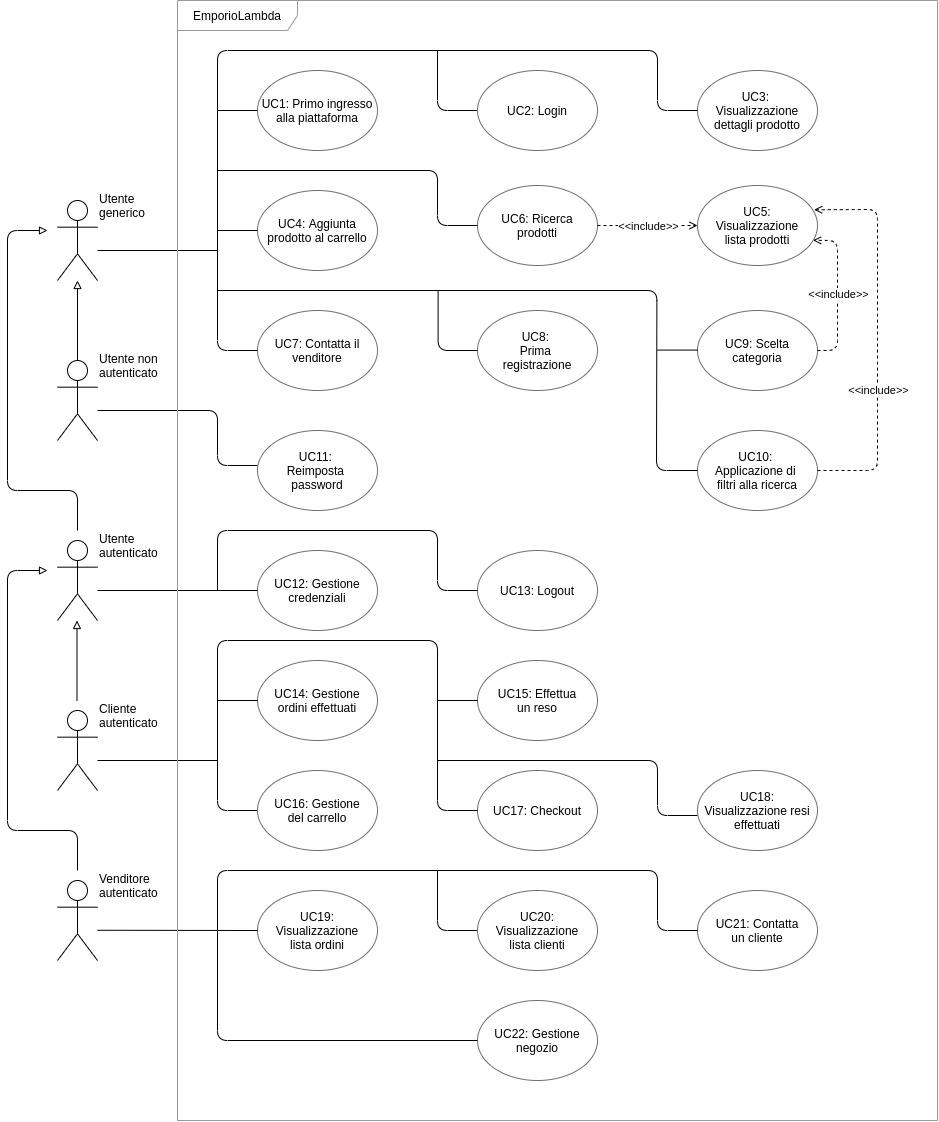
\includegraphics[scale=0.5]{../../../Images/casiUso.png}
            \centering
        \end{figure}
        \subsection{UC1: Primo ingresso alla piattaforma}
        \begin{itemize}
            \item \textbf{Descrizione} L'utente effettua il primo accesso alla piattaforma;
            \item \textbf{Attore Primario} Utente generico;
            \item \textbf{Precondizione} L'utente non sta visualizzando nulla;
            \item \textbf{Postcondizione} L'utente visualizza l'homepage della piattaforma;
            \item \textbf{Scenario Principale} L'utente arriva per la prima volta nell'e-commerce e visualizza l'homepage.
        \end{itemize}
        \subsection{UC2: Login}
        \begin{itemize}
            \item \textbf{Descrizione} Permette l'autenticazione di un utente;
            \item \textbf{Attore Primario} Utente generico;
            \item \textbf{Attore Secondario} Amazon Cognito;
            \item \textbf{Precondizione}L'utente generico non si è ancora autenticato
            \item \textbf{Input} Pressione bottone login;
            \item \textbf{Postcondizione} L'utente è autenticato;
            \item \textbf{Scenario Principale} L'utente entra nella pagina, preme il bottone per il login e viene inderizzato alla pagina di login fornita da \textit{Amazon cognito}.
        \end{itemize}
        \subsection{UC3: visualizzazione dettagli di un prodotto}
        \begin{itemize}
            \item \textbf{Descrizione} L'utente può visualizzare i dettagli di un prodotto di suo interesse;
            \item \textbf{Attore Primario} Utente generico
            \item \textbf{Precondizione} L'utente generico si trova nella pagina della lista dei prodotti;
            \item \textbf{Input} Click sul prodotto (icona, immagine, nome);
            \item \textbf{Postcondizione} L'utente visualizza i dettagli del prodotto d'interesse;
            \item \textbf{Scenario Principale} L'utente all'interno della lista dei prodotti visualizza un prodotto di suo interesse e lo apre e ne visualizza i dettagli.
        \end{itemize}
        \subsection{UC4: Aggiunta di un prodotto al carrello}
        \begin{itemize}
            \item \textbf{Descrizione} L'utente aggiunge al carrello un prodotto che intende acquistare;
            \item \textbf{Attore Primario} Utente generico;
            \item \textbf{Precondizione} L'utente generico di trova nella pagina dettagliata del prodotto;
            \item \textbf{Input} Click sul bottone di aggiunta al carrello;
            \item \textbf{Postcondizione} Il prodotto è stato aggiunto al carrello;
            \item \textbf{Scenario Principale} L'utente una volta deciso il prodotto da acquistare lo aggiunge al proprio carrello tramite l'apposito bottone.
        \end{itemize}
        \subsection{UC5: Ricerca dei prodotti}
        \begin{itemize}
            \item \textbf{Descrizione} L'utente vuole ricercare un prodotto in base ad una parola chiave; 
            \item \textbf{Attore Primario} Utente generico;
            \item \textbf{Precondizione} L'utente si trova in una pagina dedicata alla ricerca; 
            \item \textbf{Input} stringa;
            \item \textbf{Postcondizione} L'utente visualizza i prodotti corrispondenti alla parola chiave;
            \item \textbf{Scenario Principale} Un utente vuole ricercare un prodotto secondo una determinata parola chiave, gli vengo mostrati tutti i risultati della ricerca nella lista dei prodotti;
            \item \textbf{Inclusioni}
            \begin{itemize}
                \item viene visualizzata una pagina con tutti i risultati della ricerca (UC6)
            \end{itemize}
        \end{itemize}
        \subsection{UC6: Visualizzazione della lista dei prodotti}
        \begin{figure}[!ht]
            \caption{Visualizzazione della lista dei prodotti}
            \vspace{10px}
            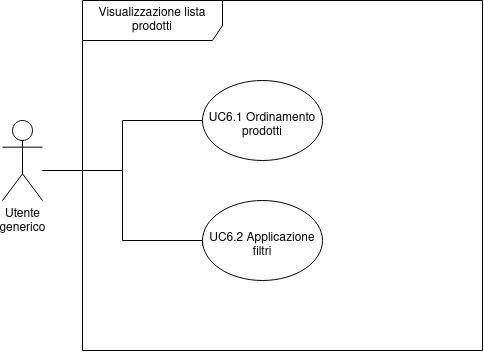
\includegraphics[scale=0.5]{../../../Images/AnalisiRequisiti/UC6.png}
            \centering
        \end{figure}
        \begin{itemize}
            \item \textbf{Descrizione} Un utente visualizza la pagina della lista dei prodotti;
            \item \textbf{Attore Primario} Utente generico;
            \item \textbf{Precondizione} L'utente non sta visualizzando nulla;
            \item \textbf{Postcondizione} L'utente visualizza la pagina con la lista dei prodotti;
            \item \textbf{Scenario Principale} L'utente arriva nella piattaforma e visualizza la lista dei prodotti;
        \end{itemize}
        \subsubsection{UC6.1: Ordinamento prodotti}
        \begin{itemize}
            \item \textbf{Descrizione} L'utente seleziona la modalità in cui visualizzare i file;
            \item \textbf{Attore Primario} Utente generico;
            \item \textbf{Precondizione} L'utente si trova all'interno di una pagina dove l'ordinamento è consentito;
            \item \textbf{Input} selezione parametro scelto
            \item \textbf{Postcondizione} La lista dei prodotti si aggiorna secondo l'ordinamento scelto;
            \item \textbf{Scenario Principale} L'utente si trova all'interno di una pagina che consente l'ordinamento, l'utente seleziona come vuole ordinare i prodotti e la pagina si aggiorna di conseguenza.
        \end{itemize}
        \subsubsection{UC6.2: Applicazione filtri}
        \begin{itemize}
            \item \textbf{Descrizione} L'utente filtra i prodotti in base alle loro caratteristiche;
            \item \textbf{Attore Primario} Utente generico
            \item \textbf{Precondizione} L'utente si trova all'interno di una pagina che consente l'utilizzo di filtri;
            \item \textbf{Input} selezione del filtro desiderato;
            \item \textbf{Postcondizione} La pagina si aggiorna secondo i filtri selezionati;
            \item \textbf{Scenario Principale} L'utente vuole filtrare i prodotti secondo determinate caratteristiche, seleziona questa e la pagina di aggiorna di conseguenza;
        \end{itemize}
        \subsection{UC7: Contatta il venditore}
        \begin{itemize}
            \item \textbf{Descrizione}
            \item \textbf{Attore Primario}
            \item \textbf{Attore Secondario}
            \item \textbf{Precondizione}
            \item \textbf{Input}
            \item \textbf{Postcondizione}
            \item \textbf{Scenario Principale}
            \item \textbf{Inclusioni}
        \end{itemize}
        \subsection{UC8: Prima registrazione}
        \begin{itemize}
            \item \textbf{Descrizione}
            \item \textbf{Attore Primario}
            \item \textbf{Attore Secondario}
            \item \textbf{Precondizione}
            \item \textbf{Input}
            \item \textbf{Postcondizione}
            \item \textbf{Scenario Principale}
            \item \textbf{Inclusioni}
        \end{itemize}
        \subsection{UC9: Scelta della categoria}
        \begin{itemize}
            \item \textbf{Descrizione}
            \item \textbf{Attore Primario}
            \item \textbf{Attore Secondario}
            \item \textbf{Precondizione}
            \item \textbf{Input}
            \item \textbf{Postcondizione}
            \item \textbf{Scenario Principale}
            \item \textbf{Inclusioni}
        \end{itemize}
        \subsection{UC10: Reimposta password (dimenticata)}
        \begin{itemize}
            \item \textbf{Descrizione}
            \item \textbf{Attore Primario}
            \item \textbf{Attore Secondario}
            \item \textbf{Precondizione}
            \item \textbf{Input}
            \item \textbf{Postcondizione}
            \item \textbf{Scenario Principale}
            \item \textbf{Inclusioni}
        \end{itemize}
        \subsection{UC12: Gestione credenziali}
        \subsection{UC13: Logout}
        \subsection{UC14: Gestione degli ordini effettuati}
        \subsection{UC15: Effettua un reso}
        \subsection{UC16: Gestione del carrello}
        \subsection{UC17: Checkout}
        \subsection{UC18: Visualizzazione dei resi effettuati}
        \subsection{UC19: Visualizzazione della lista degli ordini}
        \subsection{UC20: Visualizzazione della lista degli utenti}
        \subsection{UC21: Contatta un cliente}
        \subsection{UC22: Gestione del negozio}


\section{Requisiti}
Ogni requisito è composto dalla seguente struttura:
\begin{itemize}
    \item \textbf{Codice identificativo:} ogni codice identificativo è univoco e conforme alla seguente codifica:
          \begin{center}
              \textbf{R[ID][Tipologia]}
          \end{center}
          Il significato delle voci è:
    \item \textbf{ID:} identificatore univoco del requisito in forma gerarchica.
    \item \textbf{Tipologia:} ogni requisito può assumere uno dei seguenti valori:
          \begin{itemize}
              \item \textit{F}: funzionale;
              \item \textit{Q}: qualitativo;
              \item \textit{V}: vincolo;
              \item \textit{P}: prestazionale.
              \item
          \end{itemize}
    \item \textbf{Importanza:} riporta l'importanza del requisito:
          \begin{itemize}
              \item obbligatorio: requisito irrinunciabile per gli stakeholder;
              \item desiderabile: requisito non strettamente necessario che però apporta un valore aggiunto al prodotto;
              \item opzionale: requisito relativamente utile oppure contrabile in un secondo momento durante lo sviluppo;
          \end{itemize}
    \item \textbf{Descrizione:} descrizione del requisito, meno ambigua possibile;
    \item \textbf{Fonti:} ogni requisito deriva da una di queste fonti:
          \begin{itemize}
              \item \textit{capitolato:} è un requisito individuato dalle condizione imposte dal capitolato;
              \item \textit{interno:} è un requisito aggiunto dagli analisti;
              \item \textit{caso d'uso:} è un requisito estratto da uno o più casi d'uso, è riportato il codice del caso d'uso a cui ci si riferisce;
              \item \textit{verbale:} è un requisito individuato attraverso una riunione con i proponenti.
          \end{itemize}
\end{itemize}

\subsection{Requisiti funzionali}
\begin{center}
    %\begin{table}[!ht]
    \centering
    \rowcolors{2}{logo!10}{logo!40}
    % \setlength\extrarowheight{2pt}
    \renewcommand{\arraystretch}{1.8}
    \label{tab:RequisitiFunzionali}
    \begin{longtable}[!h]{p{50px} p{210px} p{80px} p{50px}}
        \rowcolor{logo!70} \textbf{Requisito} & \textbf{Descrizione}                                                                                & \textbf{Classificazione} & \textbf{Fonti}                               \\
        \textbf{R1F}                          & L'utente deve poter visualizzare l'homepage                                                         & Obbligatorio             & Capitolato, \newline \hyperref[sec:UC1]{UC1} \\
        R1.1F                                 & Il cliente deve poter vedere i prodotti in evidenza e in offerta                                    & Obbligatorio             & Capitolato                                   \\
        R1.2F                                 & Il cliente dalla home page deve poter accedere facilmente alla barra di ricerca e al menù           & Obbligatorio             & Capitolato                                   \\
        R1.3F                                 & Il cliente dalla home page deve poter accedere al carrello                                          & Obbligatorio             & Capitolato                                   \\
        \textbf{R2F}                          & L'utente deve poter visualizzare la pagina per l'autenticazione                                     & Obbligatorio             & \hyperref[sec:UC2]{UC2}                      \\
        \textbf{R3F}                          & L'utente deve poter autenticarsi tramite username e password                                        & Obbligatorio             & \hyperref[sec:UC3]{UC3}                      \\
        R3.1F                                 & L'utente deve poter inserire il proprio username nella pagina di autenticazione                     & Obbligatorio             & \hyperref[sec:UC3.1]{UC3.1}                  \\
        R3.2F                                 & L'utente deve poter inserire la propria password nella pagina di autenticazione                     & Obbligatorio             & \hyperref[sec:UC3.2]{UC3.2}                  \\
        \textbf{R4F}                          & L'utente deve poter autenticarsi tramite un servizio esterno                                        & Obbligatorio             & \hyperref[sec:UC4]{UC4}                      \\
        \textbf{R5F}                          & L'utente deve poter visualizzare i dettagli di un prodotto                                          & Obbligatorio             & \hyperref[sec:UC5]{UC5}                      \\
        R5.1F                                 & L'utente deve poter visualizzare il nome del prodotto                                               & Obbligatorio             & \hyperref[sec:UC5]{UC5}                      \\
        R5.2F                                 & L'utente deve poter visualizzare una foto del prodotto                                              & Obbligatorio             & \hyperref[sec:UC5]{UC5}                      \\
        R5.3F                                 & L'utente deve poter visualizzare una descrizione del prodotto                                       & Obbligatorio             & \hyperref[sec:UC5]{UC5}                      \\
        R5.4F                                 & L'utente deve poter visualizzare il prezzo del prodotto                                             & Obbligatorio             & \hyperref[sec:UC5]{UC5}                      \\
        R5.5F                                 & L'utente deve poter visualizzare l'\textit{IVA} del prodotto                                        & Obbligatorio             & Capitolato                                   \\
        R5.6F                                 & L'utente deve poter visualizzare la disponibilità del prodotto                                      & Desiderabile             & \hyperref[sec:UC5]{UC5}                      \\
        R5.7F                                 & Il cliente deve poter accedere al carrello dal dettaglio del prodotto                               & Obbligatorio             & \hyperref[sec:UC5]{UC5}                      \\
        \textbf{R6F}                          & L'utente deve poter aggiungere un prodotto al carrello                                              & Obbligatorio             & \hyperref[sec:UC6]{UC6}                      \\
        \textbf{R7F}                          & L'utente deve poter cercare i prodotti tramite una parola chiave                                    & Obbligatorio             & \hyperref[sec:UC7]{UC7}                      \\
        \textbf{R8F}                          & L'utente deve poter visualizzare la lista di prodotti                                               & Obbligatorio             & \hyperref[sec:UC8]{UC8}                      \\
        R8.1F                                 & L'utente deve poter selezionare più prodotti                                                        & Obbligatorio             & Capitolato                                   \\
        \textbf{R9F}                          & L'utente deve poter ordinare la lista di prodotti                                                   & Desiderabile             & \hyperref[sec:UC8.1]{UC8.1}                  \\
        R9.1F                                 & Il cliente deve poter ordinare i prodotti per prezzo                                                & Desidirabile             & \hyperref[sec:UC8.1]{UC8.1}                  \\
        R9.2F                                 & Il cliente deve poter ordinare i prodotti per nome                                                  & Desiderabile             & \hyperref[sec:UC8.1]{UC8.1}                  \\
        \textbf{R10F}                         & L'utente deve poter filtrare la lista di prodotti                                                   & Obbligatorio             & \hyperref[sec:UC8.2]{UC8.2}                  \\
        R10.1F                                & Il cliente deve poter decidere un prezzo minimo                                                     & Obbligatorio             & \hyperref[sec:UC8.2]{UC8.2}                  \\
        R10.2F                                & Il cliente deve poter decidere un prezzo massimo                                                    & Obbligatorio             & \hyperref[sec:UC8.2]{UC8.2}                  \\
        R10.3F                                & Il cliente deve poter filtrare per marca                                                            & Opzionale                & \hyperref[sec:UC8.2]{UC8.2}                  \\
        R10.4F                                & Il cliente deve poter filtrare per categoria                                                        & Desiderabile             & \hyperref[sec:UC8.2]{UC8.2}                  \\
        R10.5F                                & Il cliente deve poter modificare un filtri                                                          & Obbligatorio             & \hyperref[sec:UC8.2]{UC8.2}                  \\
        R10.6F                                & Il cliente deve poter rimuovere i filtri                                                            & Obbligatorio             & \hyperref[sec:UC8.2]{UC8.2}                  \\
        \textbf{R11F}                         & L'utente deve poter registrarsi inserendo i propri dati                                             & Obbligatorio             & \hyperref[sec:UC10]{UC10}                    \\
        \textbf{R12F}                         & L'utente deve poter registrarsi tramite un servizio esterno                                         & Obbligatorio             & \hyperref[sec:UC11]{UC11}                    \\
        \textbf{R13F}                         & L'utente deve poter gestire il carrello                                                             & Obbligatorio             & \hyperref[sec:UC12]{UC12}                    \\
        R13.1F                                & L'utente deve poter visualizzare i prodotti inseriti nel carrello                                   & Obbligatorio             & \hyperref[sec:UC12.1]{UC12.1}                \\
        R13.2F                                & L'utente deve poter rimuovere i prodotti inseriti nel carrello                                      & Obbligatorio             & \hyperref[sec:UC12.2]{UC12.2}                \\
        R13.3F                                & L'utente deve poter cambiare la quantità dei prodotti inseriti nel carrello                         & Desiderabile             & \hyperref[sec:UC12.3]{UC12.3}                \\
        R13.4F                                & L'utente deve essere avvisato se la quantità in magazzino è minore della quantità nel carrello      & Desiderabile             & \hyperref[sec:UC12.4]{UC12.4}                \\
        R13.5F                                & L'utente deve poter visualizzare il conto totale del carrello                                       & Obbligatorio             & Capitolato                                   \\
        R13.6F                                & L'utente deve poter visualizzare l'\textit{IVA} totale del carrello                                 & Obbligatorio             & Capitolato                                   \\
        \textbf{R14F}                         & Un utente che non riesce ad accedere deve poter reimpostare la password                             & Obbligatorio             & \hyperref[sec:UC14]{UC14}                    \\
        \textbf{R15F}                         & L'utente deve poter modificare i propri dati di profilo                                             & Obbligatorio             & \hyperref[sec:UC15]{UC15}                    \\
        R15.1F                                & L'utente deve poter modificare la propria mail di accesso                                           & Obbligatorio             & \hyperref[sec:UC15]{UC15}                    \\
        R15.2F                                & L'utente deve poter modificare il proprio username                                                  & Obbligatorio             & \hyperref[sec:UC15]{UC15}                    \\
        R15.3F                                & L'utente deve poter cambiare la propria password                                                    & Obbligatorio             & \hyperref[sec:UC15]{UC15}                    \\
        R15.4F                                & L'utente deve poter modificare il proprio nominativo                                                & Obbligatorio             & \hyperref[sec:UC15]{UC15}                    \\
        \textbf{R16F}                         & L'utente deve poter effettuare il logout                                                            & Obbligatorio             & \hyperref[sec:UC16]{UC16}                    \\
        \textbf{R17F}                         & L'utente deve poter visualizzare i propri dati di profilo                                           & Obbligatorio             & \hyperref[sec:UC17]{UC17}                    \\
        \textbf{R18F}                         & L'utente deve poter contattare il venditore                                                         & Obbligatorio             & \hyperref[sec:UC18]{UC18}                    \\
        \textbf{R20F}                         & L'utente deve poter effettuare il checkout di un ordine                                             & Obbligatorio             & \hyperref[sec:UC19]{UC19}                    \\
        R20.1F                                & L'utente deve poter inserire i dati di pagamento                                                    & Obbligatorio             & \hyperref[sec:UC19.1]{UC19.1}                \\
        R20.2F                                & L'utente deve poter inserire l'indirizzo di fatturazione                                            & Obbligatorio             & \hyperref[sec:UC19.1]{UC19.1}                \\
        R20.3F                                & L'utente deve poter inserire l'indirizzo di spedizione                                              & Obbligatorio             & \hyperref[sec:UC19.2]{UC19.2}                \\
        R20.4F                                & L'utente deve poter essere indirizzato ad un servizio per il pagamento                              & Obbligatorio             & \hyperref[sec:UC19.3]{UC19.3}                \\
        R20.5F                                & L'utente deve poter essere avvisato del mancato pagamento                                           & Obbligatorio             & \hyperref[sec:UC19.4]{UC19.4}                \\
        \textbf{R21F}                         & L'utente deve poter annullare il checkout                                                           & Obbligatorio             & \hyperref[sec:UC20]{UC20}                    \\
        \textbf{R22F}                         & L'utente deve essere indirizzato al riepilogo una volta completato l'ordine                         & Obbligatorio             & \hyperref[sec:UC21]{UC21}                    \\
        \textbf{R23F}                         & L'utente deve poter visualizzare la lista degli ordini che ha effettuato                            & Obbligatorio             & \hyperref[sec:UC22]{UC22}                    \\
        \textbf{R24F}                         & Il venditore deve poter visualizzare la lista di clienti                                            & Obbligatorio             & \hyperref[sec:UC23]{UC23}                    \\
        \textbf{R25F}                         & Il venditore deve poter visualizzare la lista degli ordini                                          & Obbligatorio             & \hyperref[sec:UC24]{UC24}                    \\
        \textbf{R26F}                         & Il venditore deve poter contattare un cliente                                                       & Obbligatorio             & \hyperref[sec:UC25]{UC25}                    \\
        \textbf{R27F}                         & Il venditore deve poter gestire i prodotti del negozio                                              & Obbligatorio             & \hyperref[sec:UC26]{UC26}                    \\
        R27.1F                                & Il venditore deve poter aggiungere un nuovo prodotto                                                & Obbligatorio             & \hyperref[sec:UC26.1]{UC26.1}                \\
        R27.2F                                & Il venditore deve poter modificare un prodotto                                                      & Obbligatorio             & \hyperref[sec:UC26.2]{UC26.2}                \\
        R27.3F                                & Il venditore deve poter rimuovere un prodotto                                                       & Obbligatorio             & \hyperref[sec:UC26.3]{UC26.3}                \\
        \textbf{R28F}                         & Il venditore deve poter gestire le categorie di prodotti                                            & Obbligatorio             & \hyperref[sec:UC27]{UC27}                    \\
        R28.1F                                & Il venditore deve poter aggiungere una nuova categoria                                              & Obbligatorio             & \hyperref[sec:UC27.1]{UC27.1}                \\
        R28.3F                                & Il venditore deve poter rimuovere una categoria                                                     & Obbligatorio             & \hyperref[sec:UC27.2]{UC27.2}                \\
        \textbf{R28F}                         & L'utente deve poter visualizzare un errore se inserisce dei dati sbagliati durante l'autenticazione & Obbligatorio             & \hyperref[sec:UC28]{UC28}                    \\
        \rowcolor{white}\caption{Rquisiti funzionali}
    \end{longtable}
    %\end{table}
\end{center}
\subsection{Requisiti di qualità}
\begin{center}
    %\begin{table}[!ht]
    \centering
    \rowcolors{2}{logo!10}{logo!40}
    % \setlength\extrarowheight{2pt}
    \renewcommand{\arraystretch}{1.8}
    \label{tab:RequisitiQualita}
    \begin{longtable}[!h]{p{50px} p{200px} p{100px} p{50px}}
        \rowcolor{logo!70} \textbf{Requisito} & \textbf{Descrizione}                                                                                                                                        & \textbf{Classificazione} & \textbf{Fonti} \\
        \textbf{R1Q}                          & Deve essere prodotta una documentazione sull'uso del sito per l'utente                                                                                      & Obbligatorio             & Capitolato     \\
        \textbf{R2Q}                          & Deve essere prodotta una documentazione sull'istallazione dell'intera infrastuttura                                                                         & Obbligatorio             & Capitolato     \\
        \textbf{R3Q}                          & Le documentazioni devono essere scritte in lingua inglese                                                                                                   & Obbligatorio             & Capitolato     \\
        \textbf{R4Q}                          & Il codice deve essere ospitato sui una repository pubblica su github                                                                                        & Obbligatorio             & Capitolato     \\
        \textbf{R5Q}                          & Il software sviluppato deve eseere coerente con quanto descritto dal documento \textit{Norme di Progetto v1.0.0}                                            & Obbligatorio             & Interno        \\
        \textbf{R6Q}                          & Tutto il codice (commenti, nomi di variabili, ecc...), commit di git, nomi di cartelle e tutto quello che rigiarda il codice deve essere scritto in inglese & Obbligatorio             & Capitolato     \\
        \textbf{R7Q}                          & Non vanno usate chiamate di \textit{callback}, ma solo funzioni \textit{awayt/async}                                                                        & Obbligatorio             & Capitolato     \\
        \textbf{R8Q}                          & Vanno definiti test di unità per ogni microservizio, distribuito su AWS                                                                                     & Obbligatorio             & Capitolato     \\
        \rowcolor{white}\caption{Rquisiti di qualità}
    \end{longtable}
    %\end{table}
\end{center}
\subsection{Requisiti di vincolo}
\begin{center}
    %\begin{table}[!ht]
    \centering
    \rowcolors{2}{logo!10}{logo!40}
    % \setlength\extrarowheight{2pt}
    \renewcommand{\arraystretch}{1.8}
    \label{tab:RequisitiVincolo}
    \begin{longtable}[!h]{p{50px} p{200px} p{100px} p{50px}}
        \rowcolor{logo!70} \textbf{Requisito} & \textbf{Descrizione}                                                                                                 & \textbf{Classificazione} & \textbf{Fonti} \\
        \textbf{R1V}                          & L'architettura dell'applicazione deve essere bastata sulla microservices architecture                                & Obbligatorio             & Capitolato     \\
        \textbf{R2V}                          & I microservizi devono essere delle funzioni \newline Lambda ospitate su \textit{AWS lambda}                          & Obbligatorio             & Capitolato     \\
        \textbf{R3V}                          & Deve essere sviluppato un componente, il \textit{BFF}, che gestistisca la comunicazione tra front-end e microservizi & Obbligatorio             & Capitolato     \\
        \textbf{R4V}                          & Il \textit{BFF} deve essere scritto in \textit{Next.js}                                                              & Obbligatorio             & Capitolato     \\
        \textbf{R5V}                          & I microservizi devono essere scritti nell'ultima versione di \textit{TypeScript}                                     & Obbligatorio             & Capitolato     \\
        \textbf{R6V}                          & Deve essere usato \textit{DynamoDb} per lo storage dei dati                                                          & Obbligatorio             & Capitolato     \\
        \textbf{R7V}                          & Deve essere usato \textit{Stripe} come servizio esterno per il pagamento                                             & Obbligatorio             & Capitolato     \\
        \rowcolor{white}\caption{Rquisiti di vincolo}
    \end{longtable}
    %\end{table}
\end{center}
\subsection{Requisiti prestazionali}
\begin{center}
    %\begin{table}[!ht]
    \centering
    \rowcolors{2}{logo!10}{logo!40}
    % \setlength\extrarowheight{2pt}
    \renewcommand{\arraystretch}{1.8}
    \label{tab:RequisitiPrestazionali}
    \begin{longtable}[!h]{p{50px} p{200px} p{100px} p{50px}}
        \rowcolor{logo!70} \textbf{Requisito} & \textbf{Descrizione}                                                                                                                                                                             & \textbf{Classificazione} & \textbf{Fonti} \\
        \textbf{R1P}                          & Rapido caricamento delle pagine                                                                                                                                                                  & Obbligatorio             & Capitolato     \\
        R1.1P                                 & Le pagine devono essere pre-caricate lato server attraverso la tecnologia \textit{Server-side Rendering (SSR)}                                                                                   & Desiderabile             & Capitolato     \\
        R1.2P                                 & Le pagine statiche, o parti statiche di esse, devono essere renderizzate in un momento precedente alla richiesta (\textit{Static Generation (SSG)}), come al momento del build dell'applicazione & Obbligatorio             & Capitolato     \\
        \textbf{R2P}                          & L'elaborazione dei filtri deve ragionevolmente veloce                                                                                                                                            & Obbligatorio             & Interno        \\
        \rowcolor{white}\caption{Requisiti prestazionali}
    \end{longtable}
    %\end{table}
\end{center}
\subsection{Tracciamento}
\subsubsection{Fonte - Requisiti}
\subsubsection{Requisito - Fonti}
\subsection{Considerazioni}

\end{document}
